% "Станет проще"

\documentclass[a4paper,12pt]{article} % тип документа

% report, book

% Рисунки
\usepackage{graphicx}
\usepackage{wrapfig}
\usepackage{lscape}

\usepackage{hyperref}
\usepackage[rgb]{xcolor}
\hypersetup{				% Гиперссылки
    colorlinks=true,       	% false: ссылки в рамках
	urlcolor=blue          % на URL
}

%  Русский язык

\usepackage[T2A]{fontenc}			% кодировка
\usepackage[utf8]{inputenc}			% кодировка исходного текста
\usepackage[english,russian]{babel}	% локализация и переносы


% Математика
\usepackage{amsmath,amsfonts,amssymb,amsthm,mathtools} 
\DeclarePairedDelimiter\abs{\lvert}{\rvert}%


\usepackage{wasysym}

%Заговолок
\author{Поляченко Юрий \\ 726}
\title{MD-моделирование воды}
\date{\today}

\begin{document} % начало документа

\clearpage\maketitle
\thispagestyle{empty}

\newpage

\section{Метод}

Прежде чем описывать результаты расчетов, скажем о методе моделирования. Моделирование проводится в lammps при Т = 25 $C^{\circ}$, P = 1 atm.

\subsection{Единицы измерения}

Используются real единицы. Чтобы сравнивать с результатами эксперимента, известными с СИ, надо перевести все в СИ. Были заданы следующие (нетривиальные) коэффециенты перевода

\begin{itemize}
\item 1 atm = $101325$ (Pa) (в отличии от 1 bar = $10^5$ Pa)
\item 1 Kcal/mole = $4184 / N_a$ (J)
\item $N_a = 6.02 \cdot 10^{23}$ (1/mole)
\end{itemize}

\subsection{Расчет погрешностей}

\subsubsection{Погрешности средних}

Дампы можно писать с любой частотой, но это не значит, что все эти <<измерения>> будут независимы и могут считаться для увеличения N в известной оценке $\sigma_x / \langle x \rangle \sim 1/\sqrt{N}$. 

За число независимых измерений, содержащихся на траектории, предложено считать $N = t_{tot} / t_{mem}$, где $t_{mem}$ - время потери кореляции между точным решением задачи коши и нашим численным интегрированием. Оно может быть оценено. Мы делали это для Л-Дж системы, и там получалось $t^d_m \sim 6-8$ ps. Здесь для верности я считал $t^d_m = 20$ ps. Тогда погрешность измеряемой величины $f(x_i, v_i, t_k)$ будет (при условии установившегося равновесия)

\begin{equation}
\sigma_f = \dfrac{\sqrt{\langle (\Delta f) ^2 \rangle}}{\sqrt{N_{uncor}}} = \dfrac{\sqrt{\langle (f_k - \langle f \rangle)^2 \rangle}}{\sqrt{t_{tot} / t^d_m}}
\end{equation}

\subsubsection{Погрешности ошибок и флуктуаций}

Хорошо бы уметь оценивать погрешность стандартного отклонения величины, т.к. std входит в теплоемкость.

Оценка погрешности ошибки величины явно сложнее чем оценка погрешности самой величины. То, что здесь написано, придумано мной и ни где не доказано (по крайне мере я о такой не слышал). 

Можно построить гистограмму попадания измеряемой величины $f(x)$ в интервалы $[y_i; y_i + dy]$. По нашему предположению оно будет гауссовым. Мы может пофитить полученную гистограмму гауссовым распределением $(\mu, \sigma)$ и пара $(\mu_0, \sigma_0)$, дающая наименьшее отклонение от гистограммы, будет теми числами, которые мы и указываем обычно в ответе $\langle f \rangle = \mu_0 \pm \sigma_0 / \sqrt{N}$. На самом деле это уже не очень определенный алгоритм, т.к. не совсем ясно, что брать за <<отклонение>> от экпериментальной гистограммы. Обычно мы берем сумму квадратов отклонений, деленных на ошибки, но это не просто потому, что так удобно считать, а потому, что мы предполагаем, что истинное значение каждого конкретного измерения тоже распределено по гауссу, и мы на самом деле максимизируем вероятность того, что при истинных параметрах $(\mu_r, \sigma_r)$ экспериментальные точки лягут так как они легли на эксперименте. Это дает произведение экспонент, у каждой из которых в показателе стоит квадрат отклонения, поэтому максимизация вероятности реализации имеющегося события равносильно минимизации суммы квадратов отклонений. 

Тут тоже надо бы пытаться максимизировать вероятность того, что при истинных нараметрах измеряемой величины $(\mu_r, \sigma_r)$ реализуется та гистограмма, которая у нас получилась. Найдем вероятность того, что при гауссовом $(\mu, \sigma)$ распределении величины $x$ реулизуется наш случай. Для конкретного интервала $[x_i; x_i + dx]$ вероятность того что измеряемое значение попало в него именно $k_i$ раз будет

\begin{equation}
P_i = p^{k_i}(x_i)(1 - p(x_i))^{(N-{k_i})} C^{N}_{k_i},
\end{equation}

где $p(x) = f(x) \cdot dx = exp(-(x - \mu)^2 / 2 \sigma^2) / \sqrt{2 \pi} \sigma \cdot dx$

Вероятность того, что в другом интервале произошло ровно $k_j$ попаданий при том, что в $i$-ом все еще $k_i$, будет $P(k_j | k_i) = (P_j \cdot P_i) / P_i = P_j$ (по $P(A|B) = P(A \cap B) / P(B)$). Тогда вероятность реализации всей гистограммы одновременно

\[
P(\mu, \sigma) = \prod_{i = 1}^{M} P_i = \prod_{i = 1}^{M} C^{N}_{k_i}  \left( \dfrac{e^{- (\Delta x_i)^2}}{\sqrt{2 \pi} \sigma} \right)^{k_i}  \left( 1 - \dfrac{e^{- (\Delta x_i)^2}}{\sqrt{2 \pi} \sigma} \right) ^{N - {k_i}}, \hspace{7pt} \Delta x_i = \dfrac{x_i - \mu}{\sigma \sqrt{2}}
\]

Я не проверял, но было бы логично, чтобы $P(\mu, \sigma)$ имела бы максимум в $P(\langle \{x\} \rangle, std[\{x\}])$. Апроксимировав $P(\mu, \sigma)$ до 2 порядка гессианом в пространстве $(\mu, \sigma)$ вблизи максимума, по идее можно оценить погрешность $\Delta(std[\{x\}])$.

Все описанное звучит логично для меня, но оно относительно сложно в исполнении, да и гарантий того, что ответ будет верный, нет. Момент $P(k_j|k_i) = P_j$ особенно сомнителен. К тому же в работе есть гораздо более серьезные проблемы, чем отсутствие обоснования погрешностей. Поэтому эта процедура не реализовывалась.

\subsection{Получение искомых величин из расчета}

Плотность расчитывается ламмпсом автоматически. Для теплоемкостей известна их связь с тепломыми флуктуациями в системе:

\begin{equation}
C_V = \dfrac{\langle (\Delta_{nvt} E_{tot}) ^2 \rangle}{k_B T^2}
\end{equation}

\begin{equation}
C_P = \dfrac{\langle (\Delta_{npt} (E_{tot} + PV)) ^2 \rangle}{k_B T^2}
\end{equation}

В обоих случаях (nvt и npt) используется термостат Нозе-Гувера. Силы термостатов выбраны типичными согласно документации ламмпса. $\tau_{P} = 1000 dt$, $\tau_{T} = 100 dt$. Их вариации проводились -- при слишком сильном термо- и баро-статировании система ведет себя неадекватно. При выходе же на стабильный режим получаемые ответы слабо зависят от силы ...статов. Используется значение по умолчанию $dt = 1$ ps. Проверено, что больше ($dt \geq 2$ ps) брать плохо - получаемые значения меняются, а меньше бессмысленно ($C_X(dt = 1ps) = C_X(dt = 0.5 ps)$).

\subsection{Методы работы с кулоном и потенциалы}

Используется 3 ламмпс-потенциала для воды

\begin{itemize}
\item lj/cut/coul/long + pppm 1.0e-5
\item lj/cut/coul/dsf, $\sim 1/R_{dump}$, 12.0
\item lj/cut/tip4p/long ... 0.15 12.0 + pppm 1.0e-5
\end{itemize}

Параметры молекулы SPC/E: $q_O = -0.8476$ e, $q_H = 0.4238$ e, $d_{OH} = 1$ \AA, $\angle(HOH) = 109.4^{\circ}$. Для удержания заданных связей использовался rattle с точностью $10^{-5}$ и максимальным количеством последовательных итераций для удовлетворения связи = 100. Параметры рекомендованы документацией. Точность - относительная ошибка в силах.  Во всех случаях параметры Л-Дж берутся по документации ламмпса $\varepsilon = 0.1550$ Kcal/mole, $\sigma = 3.1536$ \AA. В начале было проверено, что отличие ответов при этих параметрах от ответов в SPC/E модели незначительны (хотя не очевидно, с чем сравнивать). Л-Дж взаимодейсвие вводится только между атомами кислорода.

Перейдем к результатам. Анализ верности ответа будет проводится сравнением ответов друг с другом, т.к. сойтись с экспериментом не получилось.

\section{Результаты PPPM}

\subsection{Допустимый размер системы}

Как видно, делать линейный размер системы больше 5 межатомных расстояний не сильно необходимо (опять же, с чем мы сравниваем и какая точность нужна - не ясно. Было бы сравнение с экспериментом -- тогда да, а так не ясно).  Брать меньше 5 не хорошо, т.к. область обрезки Л-Дж начинает приближаться и к периодической границе, что явно плохо.

\begin{figure}[h!]
\begin{center}
\includegraphics[width=0.8\textwidth]{./pics/pppm_H_N15}
\end{center}
\caption{pppm, $N = 15^3$} \label{img:pppm_H_N15}
\end{figure}

\newpage

\begin{figure}[h!]
\begin{center}
\includegraphics[width=0.8\textwidth]{./pics/pppm_H_N10}
\end{center}
\caption{pppm, $N = 10^3$} \label{img:pppm_H_N10}
\end{figure}

\begin{figure}[h!]
\begin{center}
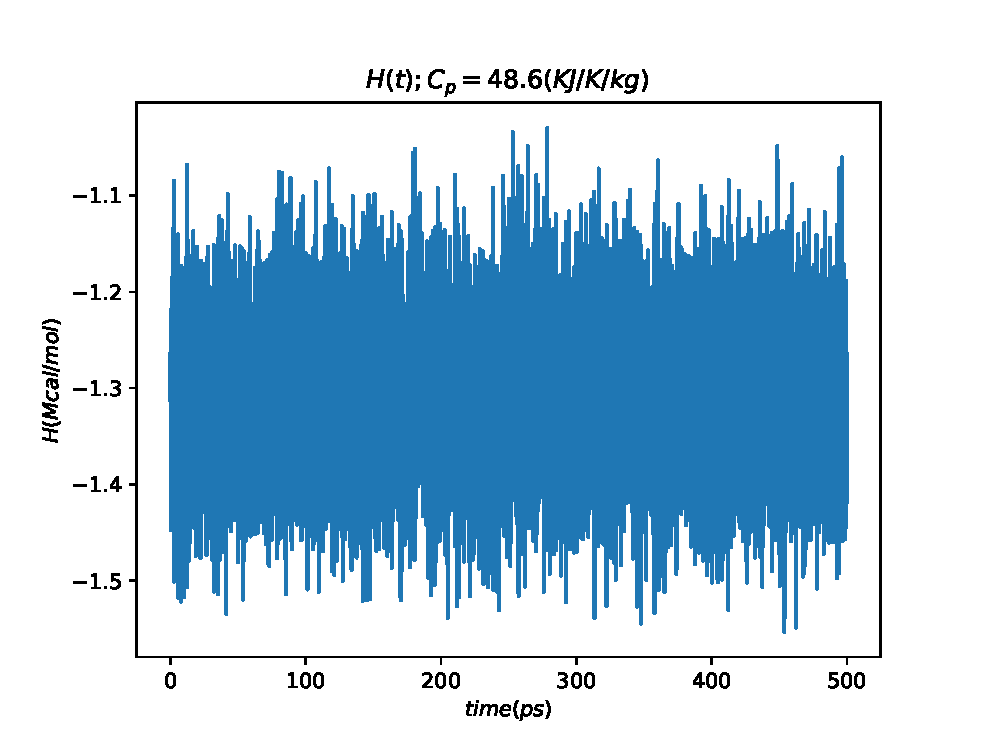
\includegraphics[width=0.8\textwidth]{./pics/pppm_H_N5}
\end{center}
\caption{pppm, $N = 5^3$} \label{img:pppm_H_N5}
\end{figure}

\newpage

\subsection{Другие равновесные характеристики}

Были измерены так же плотность, давление, полная энергия и температура системы. $C_V$ в заголовке $E_{tot}(t)$ посчитано в предположении nvt, поэтому не является релевантным, т.к. по факту расчет был npt.

\begin{figure}[h!]
\begin{center}
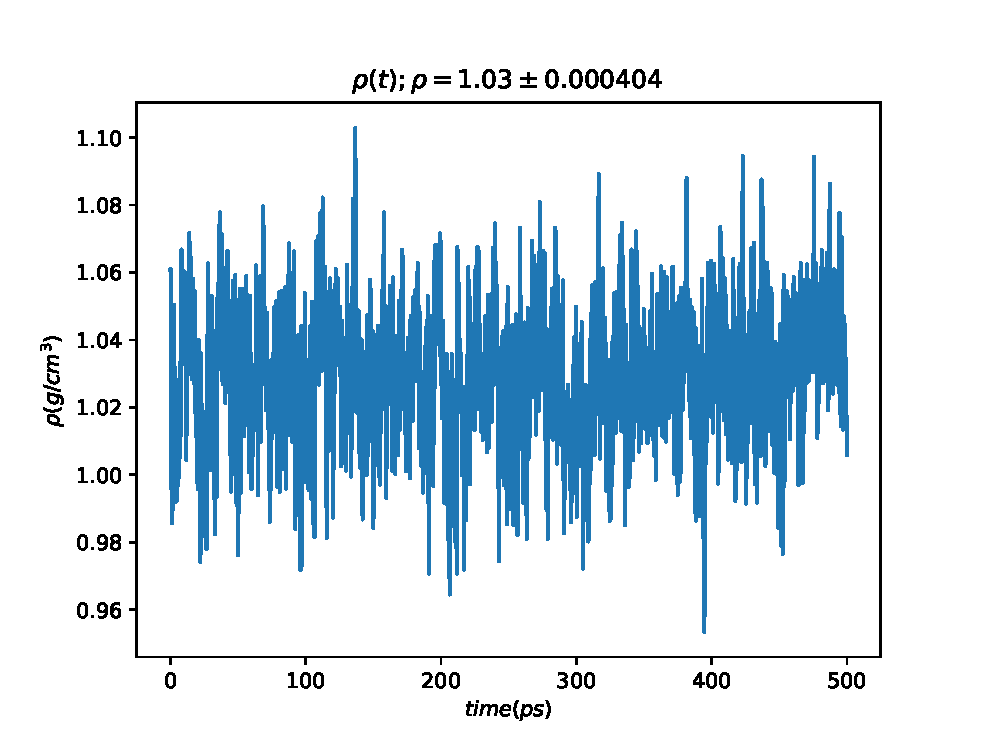
\includegraphics[width=0.68\textwidth]{./pics/pppm_N5rho}
\end{center}
\caption{pppm, $N = 5^3$} \label{img:pppm_H_N5}
\end{figure}

\begin{figure}[h!]
\begin{center}
\includegraphics[width=0.68\textwidth]{./pics/pppm_N5E}
\end{center}
\caption{pppm, $N = 5^3$} \label{img:pppm_H_N5}
\end{figure}

\newpage

\begin{figure}[h!]
\begin{center}
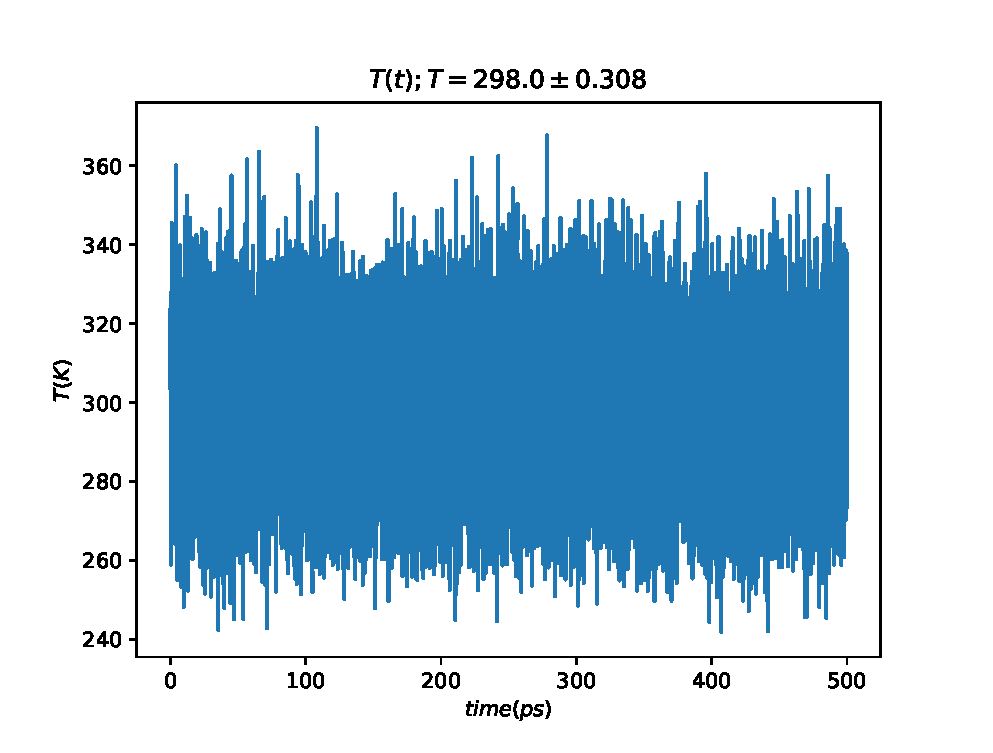
\includegraphics[width=0.8\textwidth]{./pics/pppm_N5T}
\end{center}
\caption{pppm, $N = 5^3$} \label{img:pppm_H_N5}
\end{figure}

\begin{figure}[h!]
\begin{center}
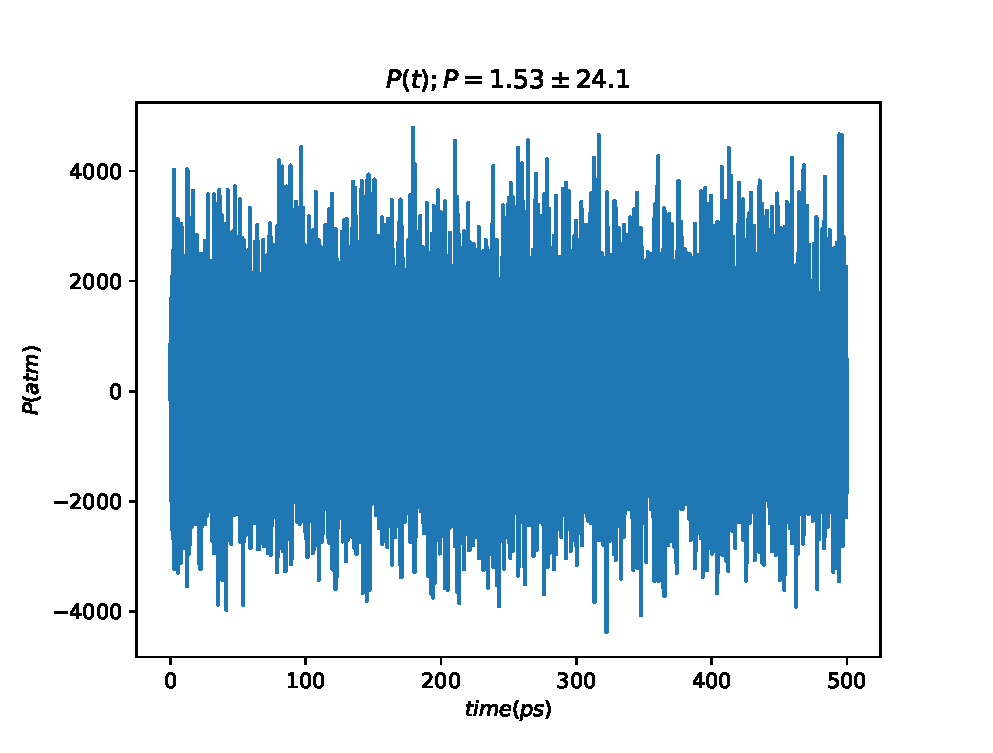
\includegraphics[width=0.8\textwidth]{./pics/pppm_N5P}
\end{center}
\caption{pppm, $N = 5^3$} \label{img:pppm_H_N5}
\end{figure}

\newpage

Можно заметить, что значение $C_V$ даже посчитанное в npt вместо положенного nvt режиме гораздо меньше отличается от экспериментального, чем значения <<правильно>> посчитанного $C_P$. Средние значение Т так же прекрасно совпадает с тем, на что был настроен термостат. В отличие от значение среднего Р, которое отличается от целевого на величину порядка себя. Из-за таких проблем с давлением я думаю, что возможно косяк в баростате, но я его пока не нашел.

\section{Результаты DSF}

Тут тоже 5 частиц в длинну ячейки оказалось достаточно для не сильного относительного отклонения теплоемкости от значений для бОльших N.

\begin{figure}[h!]
\begin{center}
\includegraphics[width=0.8\textwidth]{./pics/dsf_H_05_N15}
\end{center}
\caption{dsf, $N = 15^3$} \label{img:dsf_H_0.05_N15}
\end{figure}

\newpage

\begin{figure}[h!]
\begin{center}
\includegraphics[width=0.8\textwidth]{./pics/dsf_H_05_N10}
\end{center}
\caption{dsf, $N = 10^3$} \label{img:dsf_H_0.05_N10}
\end{figure}

\begin{figure}[h!]
\begin{center}
\includegraphics[width=0.8\textwidth]{./pics/dsf_H_05_N5}
\end{center}
\caption{dsf, $N = 5^3$} \label{img:dsf_H_0.05_N5}
\end{figure}

\subsection{Другие равновесные характеристики}

\begin{figure}[h!]
\begin{center}
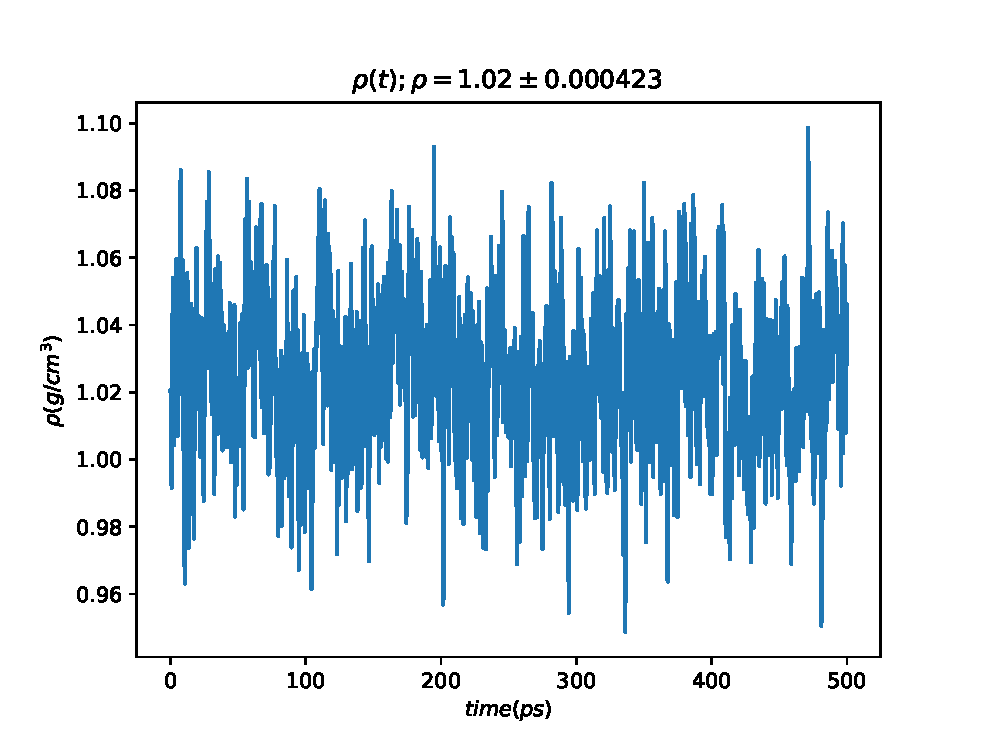
\includegraphics[width=0.68\textwidth]{./pics/dsf_N5rho}
\end{center}
\caption{dsf, $N = 5^3$} \label{img:pppm_H_N5}
\end{figure}

\begin{figure}[h!]
\begin{center}
\includegraphics[width=0.68\textwidth]{./pics/dsf_N5E}
\end{center}
\caption{dsf, $N = 5^3$} \label{img:pppm_H_N5}
\end{figure}

\newpage

\begin{figure}[h!]
\begin{center}
\includegraphics[width=0.8\textwidth]{./pics/dsf_N5T}
\end{center}
\caption{dsf, $N = 5^3$} \label{img:pppm_H_N5}
\end{figure}

\begin{figure}[h!]
\begin{center}
\includegraphics[width=0.8\textwidth]{./pics/dsf_N5P}
\end{center}
\caption{dsf, $N = 5^3$} \label{img:pppm_H_N5}
\end{figure}

\newpage

Можно заменить, что со значением кулоновского дампинга 0.05 для dsf значения теплоемсокти уже близко к значению для pppm: 48.6 vs 48.7. Можно проварьировать этот параметр, попытавшись добиться еще лучшего согласия. Для плотности результат при любых значениях, близких к значениям из документации, не меняется, так что эффективно сравниваем только $C_P$. Как видно по рисункам ниже, значение $\alpha = 0.05$ изначально было хорошим попаданием, так что можно оставить его.

\begin{figure}[h!]
\begin{center}
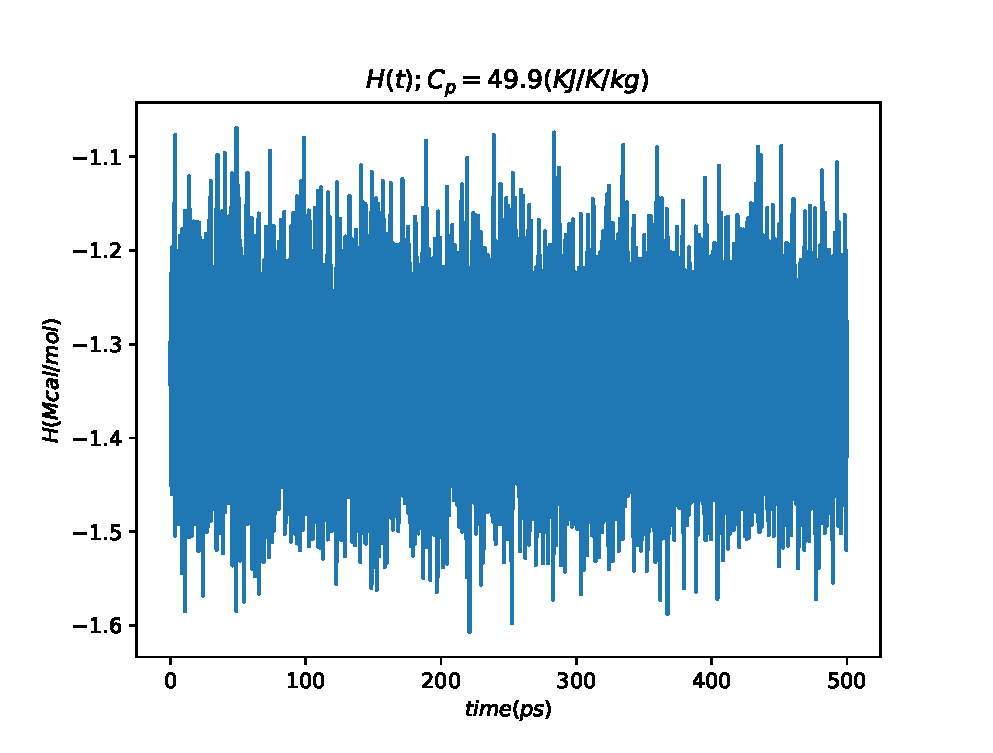
\includegraphics[width=0.8\textwidth]{./pics/e1H}
\end{center}
\caption{dsf, $\alpha = 0.1$} \label{img:pppm_H_N5}
\end{figure}

\newpage

\begin{figure}[h!]
\begin{center}
\includegraphics[width=0.8\textwidth]{./pics/e025H}
\end{center}
\caption{dsf, $\alpha = 0.025$} \label{img:pppm_H_N5}
\end{figure}

\begin{figure}[h!]
\begin{center}
\includegraphics[width=0.8\textwidth]{./pics/e055H}
\end{center}
\caption{dsf, $\alpha = 0.055$} \label{img:pppm_H_N5}
\end{figure}

\newpage

\section{Результаты tip4p}

Значения теплоемкостей расходятся с экспериментальными, поэтому для подолнительной проверки был проведен расчет с потенциалом tip4p/pppm. Тут можно отметить, что для воспроизведения результатов необходимо было заменить параметры молекулы на те, что рекомендует ламмпс. Приведем здесь это сравнение. Для $H_2 O$ из документации tip4p воспроизводит результаты, получаемые на SPC/E $H_2 O$.

\newpage

\begin{figure}[h!]
\begin{center}
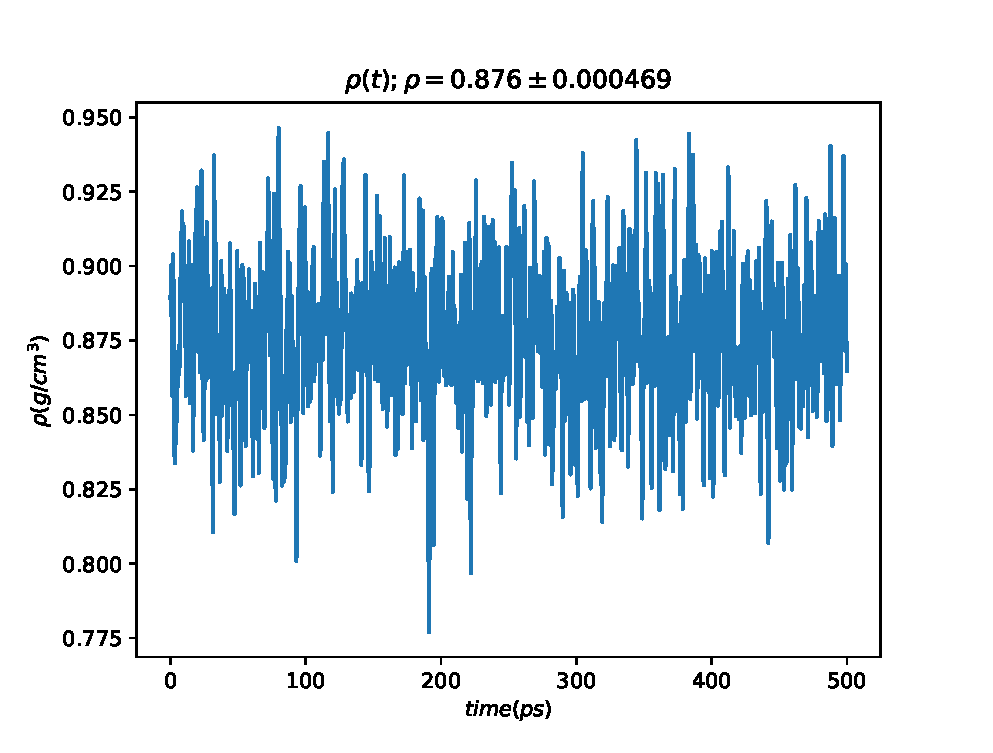
\includegraphics[width=0.8\textwidth]{./pics/stdrho}
\end{center}
\caption{tip4p/pppm, SPC/E $H_2 O$} \label{img:pppm_H_N5}
\end{figure}

\begin{figure}[h!]
\begin{center}
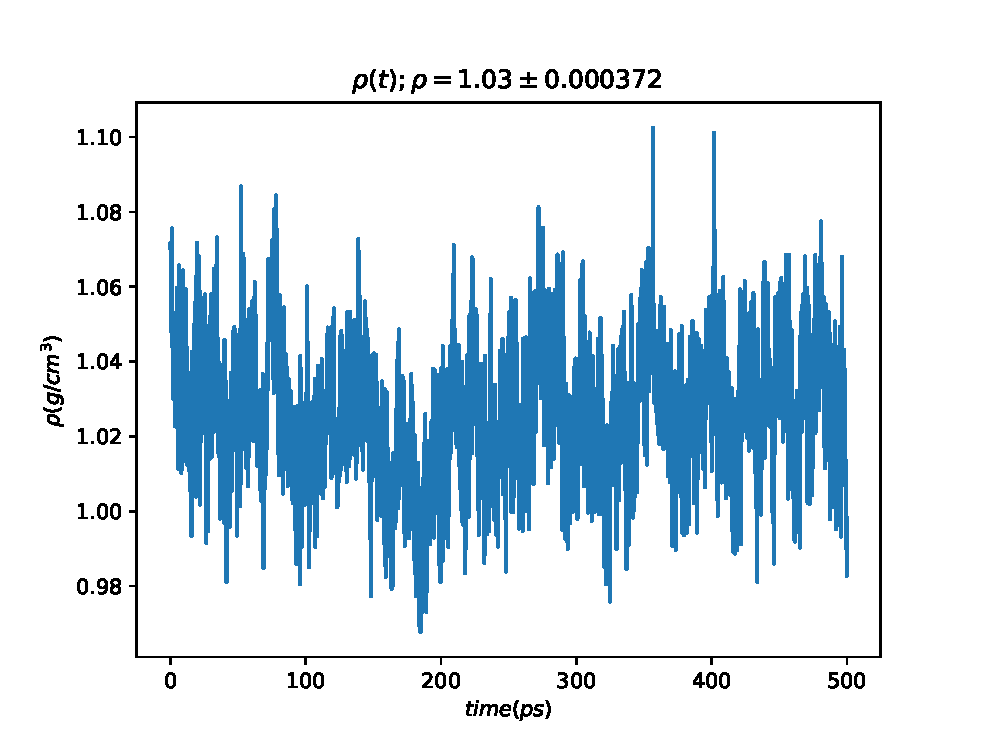
\includegraphics[width=0.8\textwidth]{./pics/tip4prho}
\end{center}
\caption{tip4p/pppm, lammps docs $H_2 O$} \label{img:pppm_H_N5}
\end{figure}

\newpage

\begin{figure}[h!]
\begin{center}
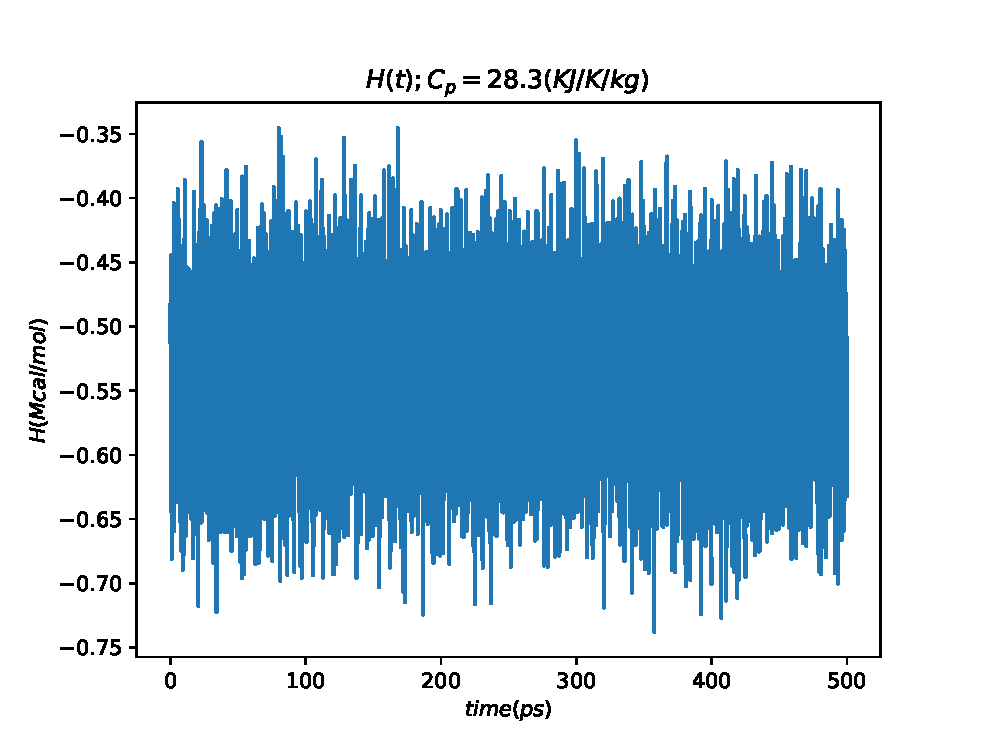
\includegraphics[width=0.8\textwidth]{./pics/stdH}
\end{center}
\caption{tip4p/pppm, SPC/E $H_2 O$} \label{img:pppm_H_N5}
\end{figure}

\begin{figure}[h!]
\begin{center}
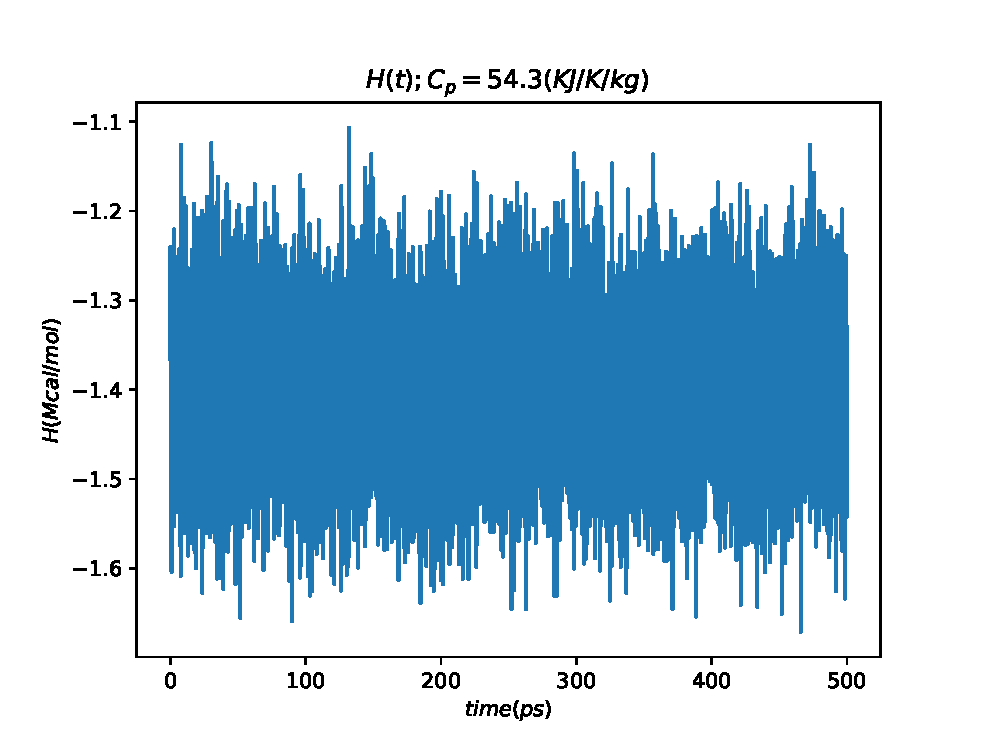
\includegraphics[width=0.8\textwidth]{./pics/tip4pH}
\end{center}
\caption{tip4p/pppm, lammps docs $H_2 O$} \label{img:pppm_H_N5}
\end{figure}

\end{document} % конец документа